%%%%%%%%%%%%%%%%%%%%%%                                              About LTU
\begin{frame}[fragile]{Deep Learning - HOW?}
LTU  : 
\textbf{Linear Threshold Unit}\\
Building blocks of neural networks
Proposed by Warren McCulloch and Walter Pitts\\
Only a concept, No learning strategy

    \begin{figure}[ht]
      \hspace*{-1cm}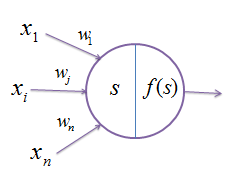
\includegraphics[width=0.5\linewidth]{ltu_image}
    \end{figure}
\end{frame}
%%%%%%%%%%%%%%%%%%%%%%                                          About Perceptron
\begin{frame}[fragile]{Deep Learning - HOW?}

Perceptron
    \begin{itemize}
        \item LTU + Learning rule .
\pause        
        \item Works only for binary classification
    \end{itemize}
    \begin{figure}[ht]
      \hspace*{-1cm}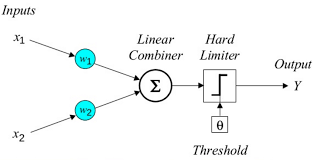
\includegraphics[width=0.5\linewidth]{ltu}
    \end{figure}
\end{frame}
%%%%%%%%%%%%%%%%%%%%%%                                          About MLP
\begin{frame}[fragile]{Deep Learning - HOW?}
    Multilayer Perceptron
    \begin{itemize}
        \item Multiple LTUs are stacked side by side and on top
\pause        
        \item Activation function : Sigmoid
    \end{itemize}
    \begin{figure}[ht]
      \hspace*{-1cm}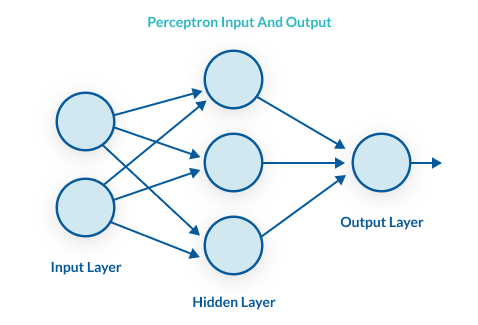
\includegraphics[width=0.5\linewidth]{mlp}
    \end{figure}
\end{frame}

%%%%%%%%%%%%%%%%%%%%%%                                          About Deep neural network
\begin{frame}[fragile]{Deep Learning - HOW?}
    Deep Neural Network \\ 
    If number of hidden layers increases
    \begin{figure}[ht]
      \hspace*{-1cm}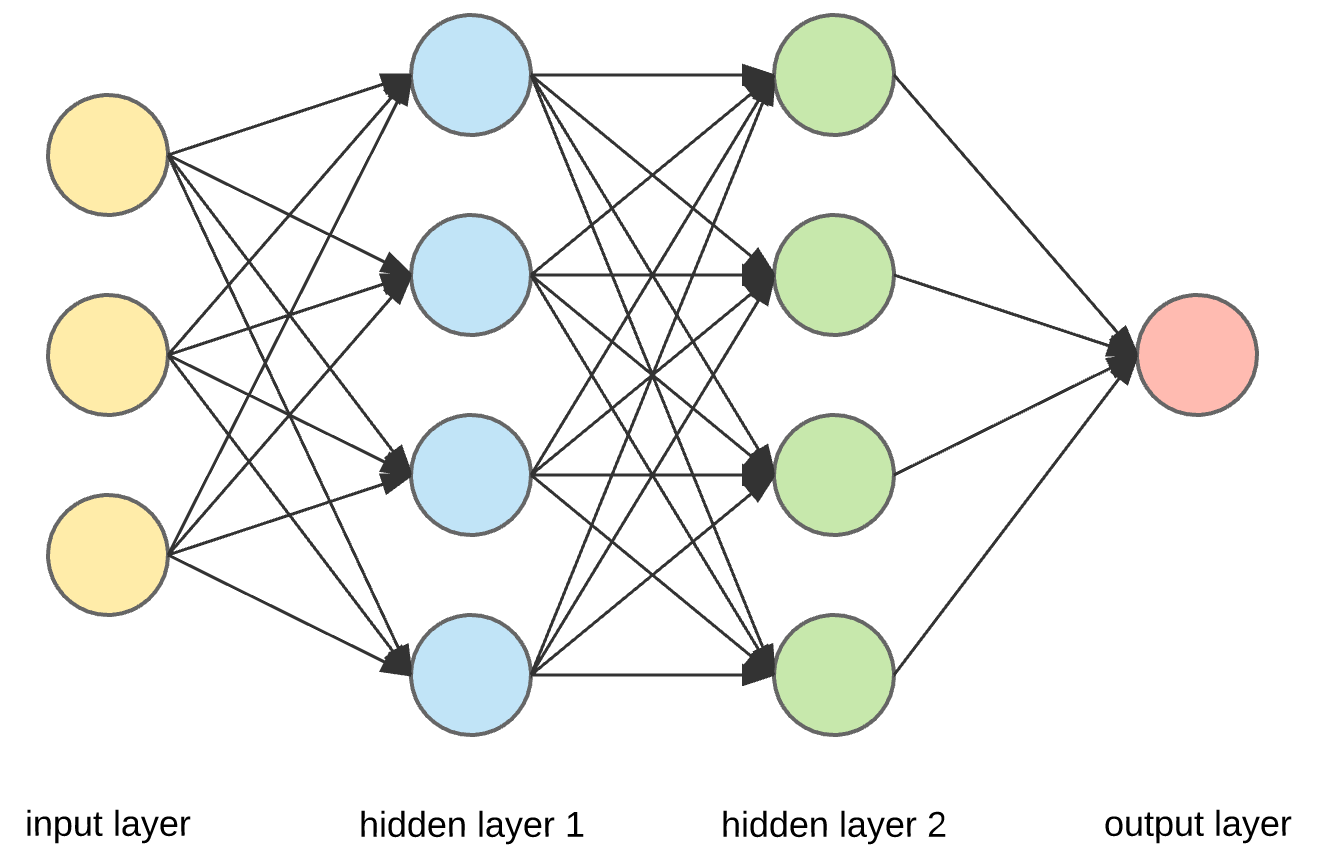
\includegraphics[width=0.5\linewidth]{dnn}
    \end{figure}
Learning Weights of a deep neurral networks is called as \textbf{deep learning}
\end{frame}

%%%%%%%%%%%%%%%%%%%%%%                                          About Convolutional layer
\begin{frame}[fragile]{Convolutional Neural Networks}
    Why \\ 
    \begin{figure}[ht]
      \hspace*{-1cm}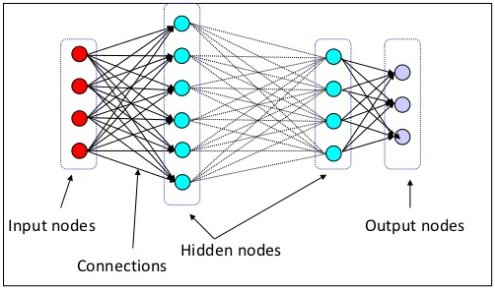
\includegraphics[width=0.5\linewidth]{conv1} \\
      \hspace*{-1cm}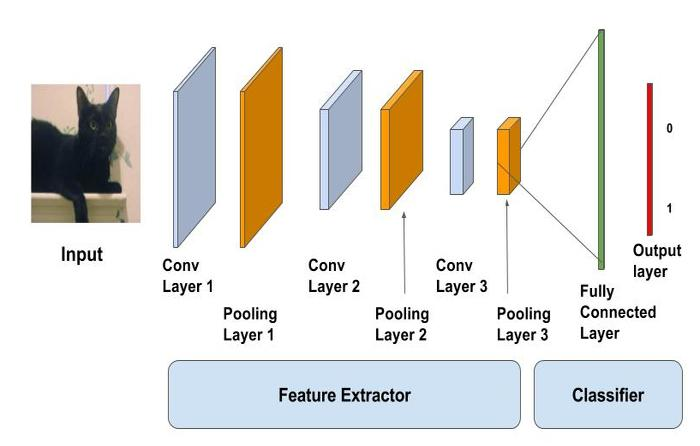
\includegraphics[width=0.5\linewidth]{conv2}
    \end{figure}
Learning Weights of a deep neurral networks is called as \textbf{deep learning}
\end{frame}

%%%%%%%%%%%%%%%%%%%%%%%%%%%%%%%%%%%%%%%%%%%%%%%%%%%%%%%%%%%%%%%%%%%%%%%%%%%%%%%%%%%%%%%%